\documentclass{article}
\usepackage[english]{babel}
\usepackage{natbib}
\usepackage{url}
\usepackage[utf8x]{inputenc}
\usepackage{amsmath}
\usepackage{graphicx}
\graphicspath{{img/}}
\usepackage{parskip}
\usepackage{fancyhdr}
\usepackage{vmargin}
\usepackage{subcaption}
\setmarginsrb{3 cm}{2.5 cm}{3 cm}{2.5 cm}{1 cm}{1.5 cm}{1 cm}{1.5 cm}

\title{MA5204: Machine Learning 2019}								% Title
\date{12 Sept 2015}											% Date

\makeatletter
\let\thetitle\@title
\let\theauthor\@author
\let\thedate\@date
\makeatother

\pagestyle{fancy}
\fancyhf{}
\rhead{\theauthor}
\lhead{\thetitle}
\cfoot{\thepage}

\begin{document}

%%%%%%%%%%%%%%%%%%%%%%%%%%%%%%%%%%%%%%%%%%%%%%%%%%%%%%%%%%%%%%%%%%%%%%%%%%%%%%%%%%%%%%%%%

\begin{titlepage}
	\centering
    \vspace*{0.5 cm}
    
\includegraphics[scale = 0.4]{logoFCFM.jpg}\\[1.0 cm]	% University Logo	% University Name
	\textsc{\LARGE Tarea 1}\\[0.5 cm]				% Course Code
	\rule{\linewidth}{0.2 mm} \\[0.4 cm]
	{ \huge \bfseries \thetitle}\\
	\rule{\linewidth}{0.2 mm} \\[1.5 cm]

	\begin{minipage}{0.4\textwidth}
		\begin{flushleft} \large
			\emph{Submitted To:}\\
			Felipe Tobar\\
			\end{flushleft}
			\end{minipage}~
			\begin{minipage}{0.4\textwidth}

			\begin{flushright} \large
			\emph{Submitted By :} \\
		  Alexandre Poupeau\\
		\end{flushright}

	\end{minipage}\\[2 cm]







\end{titlepage}

%%%%%%%%%%%%%%%%%%%%%%%%%%%%%%%%%%%%%%%%%%%%%%%%%%%%%%%%%%%%%%%%%%%%%%%%%%%%%%%%%%%%%%%%%

\pagebreak

%%%%%%%%%%%%%%%%%%%%%%%%%%%%%%%%%%%%%%%%%%%%%%%%%%%%%%%%%%%%%%%%%%%%%%%%%%%%%%%%%%%%%%%%%

\section{Verisimilitude Maximal}

We assume that the estimation of each scientist can be represented as a value obtained from a normal distribution ($Y_i \sim \mathcal{N}(\mu,\,\sigma^{2}_i)$). We assume that the mean $\mu$ is the same for each scientist and the variance $\sigma^2$ is different. \\

This describes well the problem since the scientists should have obtained the same value for the estimation (this explains why we assume there is a unique $\mu$) with little differences due to the experiment conditions (this explains why we assume the $\sigma$ are different). \\

The verisimilitude in our case can be expressed in this form :

$$l(\mu) = p(data | model) = \displaystyle \prod^n_{i=1} p(data_i|model_i) = \displaystyle \prod^n_{i=1} p(y_i|Y_i) = \displaystyle \prod^n_{i=1} \dfrac{1}{\sqrt{2\pi\sigma_i^2}} \exp(-\dfrac{1}{2\sigma_i^2}(y_i-\mu)^2)$$

We want to maximize the verisimilitude. Because $l(\mu) = p(data | model)$, saying this is the same as saying that we want to find the optimal $\mu_{opt}$ such that the probability of obtaining the data brought by the scientists assuming we know the model is the greatest.\\

However, we do not know any of the $\sigma_i$. The idea here is to calculate the sample mean (or also called empirical mean) and then to deduce the sample variance for each estimation $y_i$. We can notice that the estimations of the two first scientists seem bad based on the results of the other scientists (which is more around $\sim 9$). When not using the two first estimations to calculate the sample mean and variance we obtain the following verisimilude :

\begin{figure}[h]
  \centering
  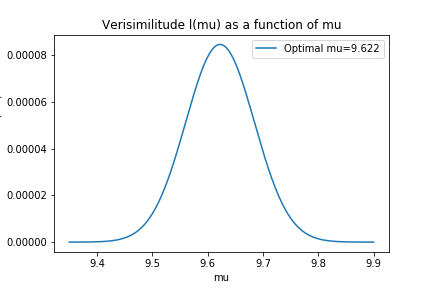
\includegraphics[scale = 0.55]{img/graph_veri_without2esti.png}
\end{figure}

Thus my conclusion is that the estimation must be around $\mu_{opt} = 9.622$. Nonetheless, we can discuss about the result. Is it a good representation  of the "true" estimation ? The answer is no for plenty of reasons. \\

The first reason is that the dataset is really small. Hence it is not possible to trust any estimation in reality when we choose the sample mean. We could imagine that the experiment is repeated $10^6$ times and that the estimations mean is around $\sim 3$. Finally, the second scientist was right but we chose to trust estimations of other scientists.\\

Another reason is that we estimate each $\sigma_i$ using a sample mean we calculated without taking into account the first and the second estimations. However, one could object that the third value is "not good" too. In this case, we would obtain $\mu_{opt} = 9.902$.\\

Another reason is that we assume we know the model. Because of the combinaison of all those reasons, the result we have is not absolutly not perfect.

\section{Lineal Regression}

\begin{figure}[h]
  \centering
  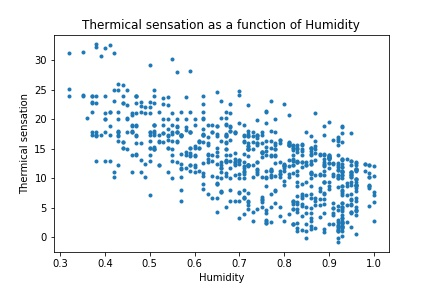
\includegraphics[scale = 0.45]{img/graph_base.jpg}
  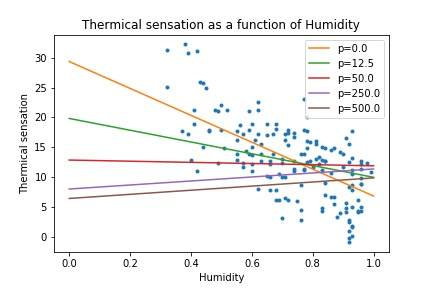
\includegraphics[scale = 0.45]{img/graph_funcp.jpg}
  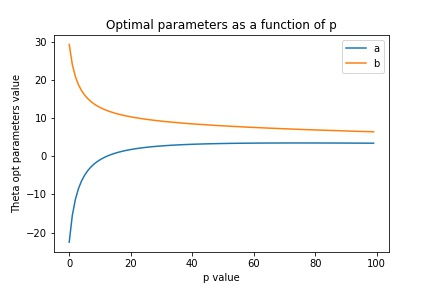
\includegraphics[scale = 0.45]{img/graph_opt_params.jpg}
  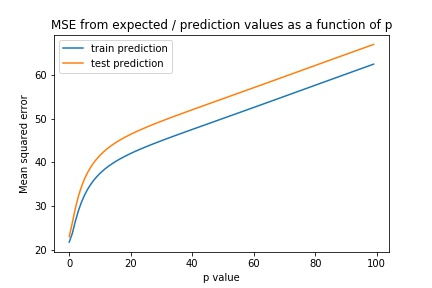
\includegraphics[scale = 0.45]{img/graph_MSE.jpg}
  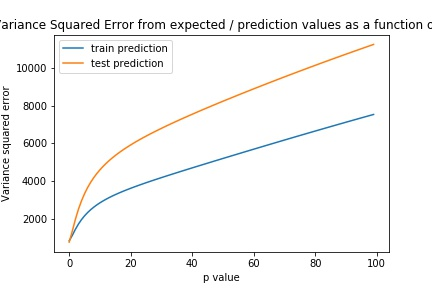
\includegraphics[scale = 0.45]{img/graph_VSE.jpg}
\end{figure}

By taking a look at all those graphs, we can deduce that the regularization affects the result in a bad way. The higher the $\rho$ value, the closer to zero are the optimal parameters. In our case, this is particularly bad because it just flattens the slope and makes the intercept closer to zero. Hence, the higher the $\rho$ value, the worse the model in our case with those data. Based on what we explained and because the problem is really simple, the regularization does not help much here. \\

The mean square error (MSE) between the test expected $Y_{exp}$ and the $Y_{pred}$ (that we can see that is greater than the MSE with the train which is expected) is minimal when $\rho = 0$ (no regularization) which confirms what we saw before. We can conclude that the lineal regression without regularization is much more efficient in this case and provides much better results.

\section{Proyecto}

I do not precisely know what is expected for the project since I could not find any information about it on U-cursos. Moreover, I do not know if we can take any subject we want or only project that can be resolved using elements we study in the course. Therefore, I propose some ideas I have found and IA projects I thought were interesting enough to go deeper :

\begin{itemize}
  \item Integer Sequence Learning : This challenges you to create a machine learning algorithm capable of guessing the next number in an integer sequence. While this sounds like pattern recognition in its most basic form, a quick look at the data will convince you this is anything but basic. I love this one, it mixes pure mathematics and machine learning (kaggle competition).
  \item Detecting insults in Social Commentary : The goal here is to predict whether a comment posted is considered insulting to one of the participants in a public discussion (kaggle competition).
  \item Reinforcement Learning : I have always wanted to work on this and know more about this topic. (idea of mine)
  \item Initial parameters in Neural Networks : Now that our society uses NN everywhere and that in many cases it takes times to train it, I asked myself if there is, for each problem, an optimal initial value for all the weights in the NN to make the training faster (idea of mine).
\end{itemize}

\cite{bibtex}

\bibliographystyle{plain}
\bibliography{biblist}

\end{document}
